% !TeX spellcheck = da_DK

Dette kapitel beskriver platformen og hvorfor den er valgt.

\section{Lego Mindstorms NXT}\label{lego:mindstorms-nxt}
I dette kapitel vil den valgte platform, \legoms, blive kort beskrevet med en begrundelse for dette valg.
Yderligere vil der blive argumenteret for valg af API til NXT-enheden.

\subsection{Hvad er Lego Mindstorms?}
\legoms er et byggesæt, hvor det er muligt at bygge programmerbare robotter i \lego-klodser.

Til at bygge disse robotter er der i \legoms nogle sensorer og aktuatorer. Sensorerne gør det muligt for robotten at modtage input fra sine omgivelser
Ved brug af aktuatorerne kan robotten reagere på disse inputs.

Ud over de originale \lego dele er der også tredjeparts forhandlere, som har et udbud af andre sensorer og aktuatorer. \thilemann{Enten bør denne linje fjernes, eller også skal vi skrive om sådanne sensorer?}

\subsubsection{Hvad er NXT?}
Denne sektion er baseret på \cite{nxt}, hvilket omhandler NXT 2.0, som er den version der bruges i dette projekt.
NXT Intelligent Brick (oftest kaldt blot 'NXT' eller 'brick') er hjernen i \legoms robotten.
Det er den der står for at modtage og behandle input fra sensorer samt styre de monterede aktuatorer.
Et billede af NXT 2.0 kan ses i \cref{platform:nxt}.

\begin{figure}
\begin{center}
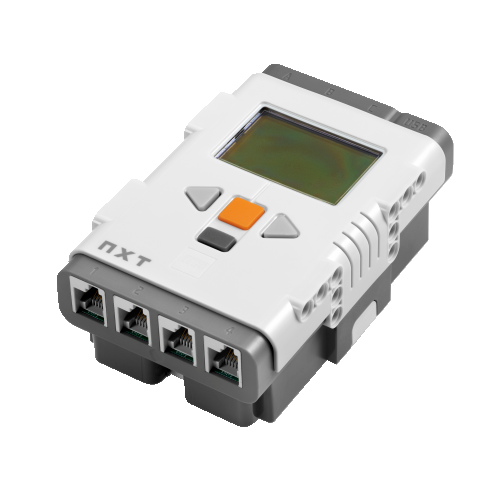
\includegraphics[scale=.5]{./graphics/nxt/brick}
\end{center}
\caption{'NXT Intelligent Brick'}
\label{platform:nxt}
\end{figure}

\subsubsection{Porte}
NXT'en har 3 motor porte (kaldet A, B og C) og 4 sensor porte (kaldet 1, 2, 3 og 4).

\subsubsection{Tilslutningsmuligheder}
Der kan kommunikeres med NXT'en ved at tilslutte den til en anden enhed med USB-kabel eller Bluetooth\textregistered.

\subsubsection{Feedback}
Til output har NXT'en en 100 x 64 pixel LCD display samt en 8 kHz højttaler.

\subsubsection{Styring}
NXT'en kan styres på to måder:
Man kan sende kommandoer og modtage beskeder (for eksempel sensor aflæsninger) på en ekstern enhed (oftest en computer eller en anden NXT).
Alternativt kan programmer sendes (via Bluetooth eller USB) til NXT'en, hvorfra de kan køres direkte, uafhængig af eksterne enheder.


\subsubsection{Tekniske specifikationer}
De tekniske specifikationer for NXT 2.0 kan ses på \cref{mindstorms:tekniske_spec} \cite{nxt}. 


\begin{figure}
\begin{tabular}{|c |c|}
\hline
Microcontroller & \shortstack{\\32-bit ARM7 microcontroller\\ 8-bit AVR controller}\\
\hline
RAM & \shortstack{ \\256 Kb FLASH, 64 Kb RAM \\ 4 Kb FLASH, 512 b RAM} \\
\hline
Kommuniation & \shortstack{ \\Bluetooth (Bluetooth Class II V2.0 compliant) \\ USB full speed port (12 Mbit/s)}\\
\hline
Input porte & 4 \\
\hline
Output porte & 3 \\
\hline
Display & 100 x 64 pixel LCD \\
\hline
Højttaler & 8 kHz lyd. 8-bit lydkanal og 2-16 kHz sample rate\\
\hline
Strømkilde & 6 AA batteries\\
\hline
\end{tabular}
\caption{LEGO MINDSTORMS NXT tekniske specifikationer}
\label{mindstorms:tekniske_spec}
\end{figure}


\subsection{Hvorfor LEGO MINDSTORMS NXT?}
Der er mange gode grunde til at vælge \legoms NXT.
Her er givet fire overordnede punkter, der vil blive gennemgået efterfølgende:

\begin{itemize}
\item{Tilgængelighed}
\item{Nemt at gå til}
\item{Stort udvalg af sensorer}
\item{Mange muligheder ift. styring}
\end{itemize}

\subsubsection{Tilgængelighed}
Grundet at \lego (inkl. \legoms) er ment til almindelige brugere, er det masseproduceret og kan derved købes forholdsvist billigt og i helt almindelige butikker (legetøjsforretninger og ofte også supermarkeder).

\subsubsection{Nemt at gå til}
Det faktum at man bygger sin robot i \lego klodser, med tilføjelse af \legoms sensorer/aktautorer gør det nemt at lave en konstruktion og derefter modificere den så den udfører sin opgave tilfredsstillende.

Denne høje versatilitet gør at \lego er perfekt til en prototype-orienteret fremgangsmåde for bygning af robotter.

\subsubsection{Stort udvalg af sensorer}
På grund af det store udvalg af sensorer kan man bygge robotter der kan løse et væld af opgaver.
Ved et projekt med høj usikkerhed, er det derved også nemt og billigt at udskifte en sensor.

\subsubsection{Mange muligheder ift. styring}
Her menes der både overordnet den måde hvorpå robotten styres, men især også den måde hvorpå NXT'en styres.
NXT'en kan udstyres med brugerdefineret firmware, der giver utroligt mange muligheder (og dermed også fleksibilitet) ift. hvordan den kan styres.
%Desuden kan der bruges et væld af programmeringssprog til at programmere NXT'en.
I \cref{nxt_api} bliver mulighederne ift. API og mulige programmeringssprog beskrevet.


\section{Valg af NXT API}
\label{nxt_api}
\bruno{Skal skrives om - så det passer med hvad vi gør nu.}

I denne sektion bliver der argumenteret for valg af API.
Først vil de forskellige afprøvede API'er blive kort præsenteret, hvorefter vores valg vil blive fremhævet.

Overordnet set er der to muligheder når det kommer til valg af API; standard eller custom firmware.
Forskellene på de to, og hvilke muligheder de giver for valg af sprog/API'er, vil blive uddybet her.

\subsection{Standard firmware}
Ens for alle API'er der benytter sig af standard firmware, er at de sender kommandoer til NXT'en for at styre robotten. \stefan{Er det sandt for alle standard firmware API'er? Også dem vi ikke har prøvet?}
Dette gør det nemt at lave et bibliotek/interface til at styre NXT'en, hvilket også er derfor der er mange muligheder til valg af sprog.

Følgende NXT platforme som benytter sig af standard firmware er blevet undersøgt:
\begin{itemize}
\item{nxt-python}
\item{Mindsqualls}
\item{ROBOTC}
\end{itemize}

\paragraph{nxt-python} er et Python interface der gør det muligt at sende kommandoer direkte til NXT'en.
For at bruge Bluetooth\textregistered{} til at kommunikere med NXT'en, skal der bruges et eksternt bibliotek. \cite{nxt-python}

\paragraph{Mindsqualls} er et .NET bibliotek, der gør det muligt at programmere til NXT'en i Common Language Interface (CLI) sprog, som \csharp, \fsharp eller VB. \cite{mindsqualls}

Yderlige kan der ved brug af Python Tools for Visual Studio (PTVS) udvides til at skrive programmer i et .NET Python sprog (som CPython eller IronPython). \cite{ptvs}

\paragraph{ROBOTC} er et IDE hvori der skrives programmer i C til at kommunikere med NXT'en. \cite{robotc}

\subsection{Custom firmware}
\bruno{Det her skal skrives om -  vi bruger følgende firmware nu: "enhanced firmware" og man kan godt ligge programmer på NXT'en selvom der er standard firmware på.}
Med custom firmware er det muligt at lægge programmer på NXT'en og køre dem direkte uden brug af en ekstern enhed.
Da det er et større projekt at lave en firmware, er der også færre muligheder end ift. standard firmware. \stefan{Hvorfor lave en ny firmware hvis den har færre muligheder end den originale?}

Der er blevet fundet to NXT platforme som benytter sig af custom firmware:
\begin{itemize}
\item{leJOS}
\item{nxtOSEK}
\end{itemize}

\paragraph{leJOS} er en lille Java Virtual Machine (JVM), som benytter et API kaldet NXJ.
leJOS firmware erstatter standard firmware'en på NXT'en, hvorefter det bliver muligt at lægge JAVA programmer ind og køre dem direkte på NXT'en. \cite{lejos}

\paragraph{nxtOSEK} er baseret på leJOS' NXJ API, og gør det muligt at skrive C eller C++ programmer og køre dem direkte på NXT'en.
Der er API'er til styring af NXT'en i både C og C++. \cite{nxtosek}

\subsection{Valg af API}

\subsubsection{Standard og custom firmware}
Custom firmware, hvor der kan sendes og køres programmer direkte på NXT'en, har en fordel ift. at det ikke er nødvendigt at spilde tid på kommunikation med en ekstern enhed.
Dette gør at der hurtigt kan aflæses input fra sensorer for at foretage beregninger på det registrerede data for at give en reaktion i form af en kommando til en motor.

Ens for dem begge er at det stadig er muligt at sende kommandoer fra en ekstern enhed, hvilket giver mere regnekraft, hvis man eksempelvis foretager udregninger på en PC.

Siden dette projekt ikke har behov for at den udviklede robot skal reagere hurtigt ift. sine omgivelser, er det ikke et krav at der skal køres programmer direkte på NXT'en.
Dette gør det valg der skal foretages i forhold til valg af NXT platform er mere baseret på hvilket sprog projektgruppen foretrækker.
\stefan{Jeg er i tvivl om argumentet med at programmer der kører på enheden kan reagere hurtigere - har vi en kilde på det?}

\paragraph{Sprog}
Eftersom der kan vælges mellem alle de præsenterede NXT platforme, er det et spørgsmål om smag og behag.\thilemann{I forhold til?}
Alle de præsenterede sprog har fordele og ulemper, men ingen af dem gør det umuligt at løse problemet.

Efter at have prøvet de forskellige muligheder, og opvejet fordele og ulemper, er valget faldet på Mindsqualls og en kombination af \csharp og \fsharp.


Mindsqualls kan benyttes med alle .NET sprog og kan derfor udvikles i Visual Studio, som gruppen allerede er bekendte med. 
Det giver også mulighed for at skrive i \csharp, hvilket gruppen allerede har en del erfaring med. 
.NET platformen gør det også muligt at benytte andre .NET sprog til dele at programmet, og \fsharp kunne her være interessant ift. til at implementere algoritmer.
\anders{Har vi brugt \fsharp til noget endnu ?}
%\begin{table}
%\begin{tabularx}{\textwidth}{|X|X|X|X|}
%\hline
%& \textbf{Sprog} & \textbf{Værktøjer} & \textbf{Firmware} \\ \hline
%\textbf{nxt-python} & Python & Ingen & Standard \\ \hline
%\textbf{Mindsqualls} & Alle CLI (.NET) sprog & Visual Studio & Standard \\ \hline
%\textbf{Mindsqualls (PTVS)} & Python (.NET-version af Python som CPython eller IronPython) & Visual Studio + Python Tools for Visual Studio (PTVS) & Standard \\ \hline
%\textbf{nxtOSEK} & C/C++ & Eclipse CDT + cygwin & Custom \\ \hline
%\textbf{ROBOTC} & C & ROBOTC (IDE) & Standard \\
%\hline
%\end{tabularx}
%\caption{Oversigt over de afprøvede API'er}
%\label{nxt:oversigt_api}
%\end{table}
